
\chapter*{Lecture 30}

\begin{recall}{}{}
\begin{itemize}
\item Course evaluation this week
\item Laplace transform of derivative
\end{itemize}
\end{recall}



\subsection{Translation in s}
If the Laplace transform $\Lapl (f)=F(s)$ exists for $s>\alpha$, then:
\begin{equation}
\Lapl (e^{at}f)= F(s-a)
\end{equation}
for $s>\alpha+a$.

This property can be proven by computing the Laplacian:
\begin{align*}
\Lapl (e^{at}f)&= \int^\infty_0 e^{-st}e^{at}f(t) dt\\
&= \int^\infty_0 e^{(a-s)t}f(t) dt\\
&=F(s-a)
\end{align*}

\textbf{Recall:}
\begin{align*}
\boxed{\Lapl \left(f'(t)\right)= s\Lapl(f)-f(0)= sF(s)-f(0)}
\end{align*}
\begin{align*}
\boxed{\Lapl \left(f''(t)\right)= s^2F(s)-s f(0)-f'(0)}
\end{align*}


\begin{exmp}{LT ODE :}\\
Solve:
\begin{align*}
f''+3f'+2f=0 \qquad \qquad \text{with } &f(0)=0; \\
&f'(0)=1
\end{align*}
(Auxiliaury equation: $f(t)=e^{-t}+e^{-2t}$)

\textbf{Solution}\\
\begin{enumerate}
\item Take the LT of both sides:
\begin{align*}
\qquad & \Lapl(f''+3f'+2f)=\Lapl(0)\\
&=\Lapl(f'')+3\Lapl(f')+2\Lapl(f) \qquad \text{(principle of linearity)}\\
&=\underbrace{s^2 F(s) - sf(0)-f'(0)}_{\Lapl{f''}} +3\underbrace{(sF(s) - f(0))}_{\Lapl{f'}} +2F(s)\\
&=s^2 F(s) - s(0)-(1) +3(sF(s) - (0)) +2F(s)\\
&=s^2 F(s) -1 +3sF(s) +2F(s)\\
&=(s^2 +3s+2) F(s) -1 =0\\
\end{align*}
Therefore:
\begin{align*}
F(s)=\frac{1}{s^2 +3s+2}
\end{align*}
We recall that $F(s)$ corresponds to the solution $f(t)$ in the $s$-domain,

\item Find $f(t)$ using $F(s)$ using the \textbf{inverse LT}
\begin{align*}
f(t)=\Lapl^{-1}\left[F(s)\right]=\Lapl^{-1}\left[\frac{1}{s^2 +3s+2}\right]
\end{align*}
\end{enumerate}
\end{exmp}


\begin{figure}[h!]
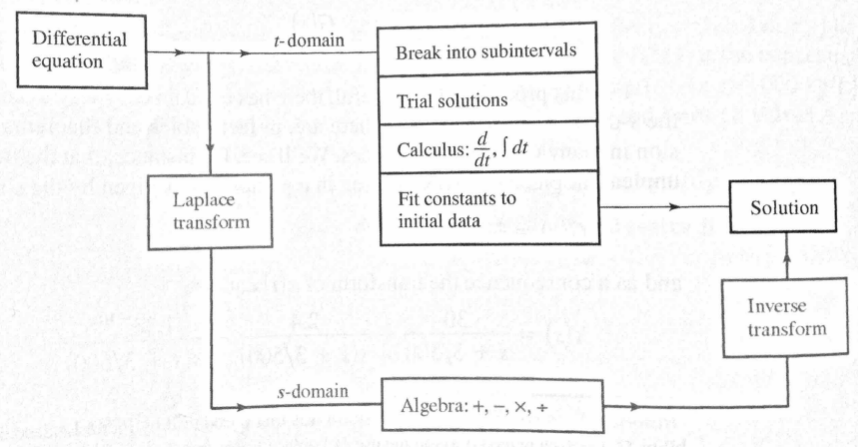
\includegraphics[width=\textwidth]{figs/LaplaceExample.png} 
\caption{Solution methods}
\end{figure}



\subsection{Definition of inverse LT}
For a given function, $F(s)$, if there is a function $f(t)$ that is continuous on $[0,\infty$ and satisfies $\Lapl\left[f(t)\right]=F(s)$, then $f(t)$ is the inverse LT of $F(s)$.\par
How do we find the inverse LT? Look up in the table! 
 \begin{figure}
\centering
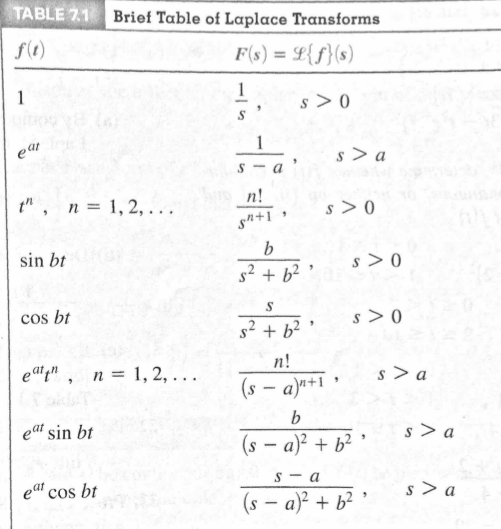
\includegraphics[width=0.7\textwidth]{figs/LaplaceIdentities.png}  
\caption{Laplace transforms}
\end{figure}




\begin{exmp}{Inverse LT:}\\
Find the inverse LT of $F(s)=\frac{1}{s^3}$. (or: $\Lapl^{-1}\left[\frac{1}{s^3}\right]$)\\
\textbf{Solution:}\\
Look up in the table, we find:
\begin{align*}
\Lapl^{-1}\left[\frac{n!}{s^{n+1}}\right]=t^n \qquad \rightarrow \Lapl^{-1}\left[\frac{1}{s^{n+1}}\right]=\frac{t^n}{n!}
\end{align*}
($n!$: n-factorial)\\
let $n+1=3$ or $n=2$
\begin{align*}
\Lapl^{-1}\left[\frac{1}{s^{3}}\right]=\frac{t^2}{2!}=\frac{t^2}{2}
\end{align*}
\end{exmp}




\begin{exmp}{Inverse LT:}\\
Find the inverse LT of $F(s)=\frac{1}{s^2+4}$.\\
\textbf{Solution:}\\
Look up in the table, we find:
\begin{align*}
&\Lapl^{-1}\left[\frac{b}{s^2+b^2}\right]=\sin(b t)\\
&\Lapl^{-1}\left[\frac{1}{s^2+b^2}\right]=\frac{\sin(b t)}{b}
\end{align*}
let $b^2=4$ or $b=2$ (we are considering the domain $[0,\infty$)
\begin{align*}
\Lapl^{-1}\left[\frac{1}{s^{2}+4}\right]=\frac{1}{2}\sin(2t)
\end{align*}

\end{exmp}

\section{Properties of the inverse LT}
It is a linear operator, therefore:
\begin{align*}
\Lapl^{-1}\left[aF(s)+bG(s)\right]=a\Lapl^{-1}\left[F(s)\right]+b\Lapl^{-1}\left[G(s)\right]
\end{align*}

\begin{exmp}{Properties of inverse LT:}\\
Find $f(t)$ if:
\begin{align*}
\Lapl^{-1}\left[\frac{5}{s-6}-\frac{6s}{s^2+9}\right]=5\Lapl^{-1}\left[\frac{1}{s-6}\right]-6\Lapl^{-1}\left[\frac{s}{s^2+9}\right]
\end{align*}
From the table, we have:
\begin{align*}
\Lapl^{-1}\left[\frac{1}{s-a}\right]=e^{at} \qquad \text{where } &a=6\\
\Lapl^{-1}\left[\frac{s}{s^2+b^2}\right]=\cos(bt) \qquad \text{where } & b=3
\end{align*}

Therefore:
\begin{align*}
\boxed{f(t)=\Lapl^{-1}\left[F(s)\right]=5e^{6t} -6\cos(3t)}
\end{align*}
\end{exmp}

\begin{center}
\line(1,0){250}
\end{center}

Suppose we have:
\begin{align*}
f(t)=\Lapl^{-1}\left[\frac{1}{s^2+3s+2}\right]
\end{align*}
Here $F(s)$ is not found in the table! What do we do?\\
\textbf{Partial fractions}!\\

Recall previous example:
\begin{align*}
\Lapl^{-1}\left[\frac{1}{s^2+3s+2}\right]=\Lapl^{-1}\left[\frac{1}{s+2}\cdot \frac{1}{s+1}\right]\stackrel{?}{=}\Lapl^{-1}\left[\frac{1}{s+2}\right]\cdot \Lapl^{-1}\left[\frac{1}{s+1}\right]
\end{align*}
This is NOT valid!! We need to create partial fractions such that:
\begin{align*}
\Lapl^{-1}\left[\frac{1}{s+2}\cdot \frac{1}{s+1}\right]=\Lapl^{-1}\left[\frac{A}{s+1}+\frac{B}{s+2}\right]=\Lapl^{-1}\left[\frac{A}{s+1}\right]+\Lapl^{-1}\left[\frac{B}{s+2}\right]
\end{align*}
We need to determine $A$ and $B$.\\
\begin{align*}
\frac{1}{(s+2)(s+1)}=\frac{A}{s+1}+\frac{B}{s+2}=\frac{A(s+2)+B(s+1)}{(s+2)(s+1)}=\frac{(A+B)s+2A+B}{(s+2)(s+1)}
\end{align*}
We know that :
\begin{align*}
A+B=0\qquad 2A+B=1 \qquad \text{or } A=1; B=-1
\end{align*}
Therefore (recall $\Lapl(e^{at})=\frac{1}{s-a}$):
\begin{align*}
f(t)&=\Lapl^{-1}\left[\frac{1}{s^2+3s+2}\right]=\Lapl^{-1}\left[\frac{1}{s+2}\right]+\Lapl^{-1}\left[\frac{-1}{s+1}\right]\\
f(t)&=e^{-t}-e^{-2t}
\end{align*}






